\usepackage{fixltx2e}
\usepackage{letltxmacro}
\usepackage{expl3}
\usepackage{xparse}
\usepackage{luacode}
\usepackage{luatexbase}
\RequireLuaModule{lualibs}
\usepackage{metalogo}

\usepackage{xcolor}
\usepackage{luacolor}

\usepackage[ngerman]{babel}
\usepackage[ngerman]{translator}
\usepackage[backend=biber,sortlocale=de_DE.UTF-8,sorting=none]{biblatex}
\usepackage[notbib,nottoc]{tocbibind}

\usepackage[sumlimits,intlimits,namelimits]{amsmath}
\usepackage{amssymb}
\usepackage{upref}
\usepackage{mathtools}
\usepackage[no-math]{fontspec} % after amssymb
\usepackage[italic,noss]{hepnicenames} % loads bm, before unicode-math
\usepackage[math-style=ISO,bold-style=ISO,sans-style=italic,nabla=upright,partial=upright,vargreek-shape=unicode,warnings-off={mathtools-colon}]{unicode-math}
\usepackage[retainorgcmds]{IEEEtrantools}
\usepackage{tensor}
\usepackage[version=3]{mhchem}
\usepackage{siunitx}
\usepackage{esvect}

\usepackage{pdflscape}
\usepackage{float}
\usepackage[above,below,section]{placeins}
\usepackage{flafter}
\usepackage[margin=10pt,font=small,labelfont=bf]{caption}
\usepackage{subcaption}
%\usepackage{subfig}
\usepackage{graphicx}
\usepackage{array}
\usepackage{multirow}
\usepackage{booktabs}

\usepackage[stable,bottom,hang]{footmisc}
\usepackage[strict]{csquotes}
\usepackage{hyphenat}
\usepackage{textcmds}
\usepackage{xspace}
\usepackage{eurosym}
%\usepackage{minted}

% Tikz %%%%%%%%%

\usepackage{tikz}
\usetikzlibrary{calc}
\usetikzlibrary{positioning}
\usetikzlibrary{shapes.geometric}
\usetikzlibrary{circuits.logic.IEC,circuits.ee.IEC}
\usetikzlibrary{arrows,shapes}
\usetikzlibrary{trees}
\usetikzlibrary{calc,through}
\usetikzlibrary{decorations.pathmorphing}	% For Feynman Diagrams
\usetikzlibrary{decorations.markings}

\pgfdeclaredecoration{complete sines}{initial}
{
    \state{initial}[
        width=+0pt,
        next state=upsine,
        persistent precomputation={\pgfmathsetmacro\matchinglength{
            \pgfdecoratedinputsegmentlength / int(\pgfdecoratedinputsegmentlength/\pgfdecorationsegmentlength)}
            \setlength{\pgfdecorationsegmentlength}{\matchinglength pt}
        }] {}
    \state{upsine}[width=\pgfdecorationsegmentlength,next state=downsine]{
        \pgfpathsine{\pgfpoint{0.50\pgfdecorationsegmentlength}{0.5\pgfdecorationsegmentamplitude}}
        \pgfpathcosine{\pgfpoint{0.50\pgfdecorationsegmentlength}{-0.5\pgfdecorationsegmentamplitude}}
    }
    \state{downsine}[width=\pgfdecorationsegmentlength,next state=upsine]{
        \pgfpathsine{\pgfpoint{0.50\pgfdecorationsegmentlength}{-0.5\pgfdecorationsegmentamplitude}}
        \pgfpathcosine{\pgfpoint{0.50\pgfdecorationsegmentlength}{0.5\pgfdecorationsegmentamplitude}}
}
    \state{final}{}
}

\tikzset{
	% >=stealth', %%  Uncomment for more conventional arrows
    vector/.style={decorate, decoration={complete sines,segment length=6}, draw},
	  provector/.style={decorate, decoration={snake,amplitude=2.5pt}, draw},
	  antivector/.style={decorate, decoration={snake,amplitude=-2.5pt}, draw},
    fermion/.style={draw=black, postaction={decorate},
        decoration={markings,mark=at position .55 with {\arrow[draw=black]{>}}}},
    fermionbar/.style={draw=black, postaction={decorate},
        decoration={markings,mark=at position .55 with {\arrow[draw=black]{<}}}},
    fermionnoarrow/.style={draw=black},
    gluon/.style={decorate, draw=black,
        decoration={coil,amplitude=4pt, segment length=5pt}},
    scalar/.style={dashed,draw=black, postaction={decorate},
        decoration={markings,mark=at position .55 with {\arrow[draw=black]{>}}}},
    scalarbar/.style={dashed,draw=black, postaction={decorate},
        decoration={markings,mark=at position .55 with {\arrow[draw=black]{<}}}},
    scalarnoarrow/.style={dashed,draw=black},
    electron/.style={draw=black, postaction={decorate},
        decoration={markings,mark=at position .55 with {\arrow[draw=black]{>}}}},
	bigvector/.style={decorate, decoration={snake,amplitude=4pt}, draw},
}
\tikzstyle{block} = [draw, rectangle, 
    minimum height=3em, minimum width=6em]


%%%%%%%%%%%%%%%%

\usepackage[unicode=true,pdfcreator={},pdfproducer={}]{hyperref}
%\usepackage{bookmark}
\usepackage[shortcuts]{extdash} % must be after hyperref for shortcuts
\usepackage{listings}


\input{modules/base.tex}
\input{modules/comment.tex}
\input{modules/floats.tex}
\input{modules/math.tex}
\input{modules/tikz.tex}
\input{modules/units.tex}

\ExplSyntaxOn

%patch maybe for hepnames
\RenewDocumentCommand \maybebm {m}
{
  \ensuremath{{{#1}}}
}
\RenewDocumentCommand \maybesf {m}
{
  \ensuremath{{#1}}
}
\RenewDocumentCommand \mayberm {m}
{
  \ensuremath{{\mathrm{#1}}}
}
\RenewDocumentCommand \maybeitrm {m}
{
  \ensuremath{{\mathrm{#1}}}
}
\RenewDocumentCommand \maybeitsubscript {m}
{
  \ensuremath{{#1}}
}

\setmainfont[BoldFont = {LMRoman10-Bold}, % not optimal
             ItalicFont = {LMRoman10-Italic}, % not optimal
             BoldItalicFont = {LMRoman10-BoldItalic}, % not optimal
             SmallCapsFont = {Latin Modern Roman Caps},
             SlantedFont = {Latin Modern Roman Slanted},
             ItalicFeatures  = {
               SmallCapsFont = {LMRomanCaps10-Oblique}
             },
            ]{Latin Modern Roman}

\setsansfont{Latin Modern Sans}

\setmonofont[SmallCapsFont = {Latin Modern Mono Caps},
             SlantedFont = {Latin Modern Mono Slanted},
             ItalicFeatures  = {
               SmallCapsFont = {LMMonoCaps10-Oblique}
             },
            ]{Latin Modern Mono}

\RenewDocumentCommand\hangfootparskip{}{0pt}
\RenewDocumentCommand\hangfootparindent{}{15pt}

\mathtoolsset{mathic}

\setmathfont{Latin Modern Math}

\setmathfont[range={\mathscr,\mathbfscr}]{XITS Math}
%\setmathfont[range={\mathcal,\mathbfcal},StylisticSet=1]{XITS Math}
\setmathfont[range={\mathcal,\mathbfcal}]{Latin Modern Math}

% much nicer than latin Modern or XITS
\DeclareSymbolFont{AMSb}{U}{msb}{m}{n}
\protected\def\mathbb#1{{\mathchar\numexpr256*\symAMSb+`#1\relax}}

% define fallbacks here
\setmathfont[range=\vDash]{XITS Math}
\setmathfont[range=\coloneq]{XITS Math}
\setmathfont[range=\propto]{XITS Math}
\setmathfont[range={\lblkbrbrak,\rblkbrbrak}]{XITS Math}

% make bar horizontal, use \hslash for slashed h
\let\hbar\relax
\DeclareMathSymbol{\hbar}{\mathord}{AMSb}{"7E}

\NewDocumentCommand \mathdefault {}
{
  \mathit
}

%\RenewDocumentCommand \header_math_tensor_font {}
%{
%  \mathit
%}

%\removenolimits{\int}
%\removenolimits{\iint}
%\removenolimits{\iiint}
%\removenolimits{\iiiint}
%\removenolimits{\oint}
%\removenolimits{\oiint}
%\removenolimits{\oiiint}
%\removenolimits{\intclockwise}
%\removenolimits{\varointclockwise}
%\removenolimits{\ointctrclockwise}
%\removenolimits{\sumint}
%\removenolimits{\intbar}
%\removenolimits{\intBar}
%\removenolimits{\fint}
%\removenolimits{\cirfnint}
%\removenolimits{\awint}
%\removenolimits{\rppolint}
%\removenolimits{\scpolint}
%\removenolimits{\npolint}
%\removenolimits{\pointint}
%\removenolimits{\sqint}
%\removenolimits{\intlarhk}
%\removenolimits{\intx}
%\removenolimits{\intcap}
%\removenolimits{\intcup}
%\removenolimits{\upint}
%\removenolimits{\lowint}

% make delimiters always grow, never have two levels the same size
\setlength{\delimitershortfall}{-1sp}

% add more space between equations, default is 3pt
\setlength{\IEEEnormaljot}{10pt}

\sisetup
{
  strict,
  locale=US,
  per-mode=symbol-or-fraction,
  separate-uncertainty=true,
  add-integer-zero=true,
  add-decimal-zero=true,
  round-integer-to-decimal=true,
  table-align-exponent=true,
  table-align-uncertainty=true,
  table-unit-alignment=center,
  math-ohm=\mathup{\Omega},
  text-ohm=\ensuremath{\mathup{\Omega}}
}

\hypersetup{
  unicode=true,
  pdfcreator={},
  pdfproducer={},
}

\addbibresource{main.bib}

\nocite{numpy, scipy, matplotlib, uncertainties, root, roofit}

\NewDocumentCommand \makebibliography {}
{
  \printbibliography[heading=bibintoc]
}

\ExplSyntaxOff


\DeclareRobustCommand{\PKst}{\HepParticle{K}{}{\ast0}\xspace}

\newcommand{\difference}[1]{\mathrm{\Delta} #1}

\title[Flavour tagging calibration]{Flavour tagging calibration of the SS\Pgp-Tagger with \HepProcess{\PBz\to\PJpsi\PKst} decays at the LHCb experiment}
\subtitle{Bachelor presentation}
\author{Igor Babuschkin}
\institute{TU Dortmund}

\newcommand{\Vud}{V_{\Pqu\Pqd}}
\newcommand{\Vus}{V_{\Pqu\Pqs}}
\newcommand{\Vub}{V_{\Pqu\Pqb}}
\newcommand{\Vcd}{V_{\Pqc\Pqd}}
\newcommand{\Vcs}{V_{\Pqc\Pqs}}
\newcommand{\Vcb}{V_{\Pqc\Pqb}}
\newcommand{\Vtd}{V_{\Pqt\Pqd}}
\newcommand{\Vts}{V_{\Pqt\Pqs}}
\newcommand{\Vtb}{V_{\Pqt\Pqb}}

\pgfdeclaredecoration{complete sines}{initial}
{
    \state{initial}[
        width=+0pt,
        next state=upsine,
        persistent precomputation={\pgfmathsetmacro\matchinglength{
            \pgfdecoratedinputsegmentlength / int(\pgfdecoratedinputsegmentlength/\pgfdecorationsegmentlength)}
            \setlength{\pgfdecorationsegmentlength}{\matchinglength pt}
        }] {}
    \state{upsine}[width=\pgfdecorationsegmentlength,next state=downsine]{
        \pgfpathsine{\pgfpoint{0.50\pgfdecorationsegmentlength}{0.5\pgfdecorationsegmentamplitude}}
        \pgfpathcosine{\pgfpoint{0.50\pgfdecorationsegmentlength}{-0.5\pgfdecorationsegmentamplitude}}
    }
    \state{downsine}[width=\pgfdecorationsegmentlength,next state=upsine]{
        \pgfpathsine{\pgfpoint{0.50\pgfdecorationsegmentlength}{-0.5\pgfdecorationsegmentamplitude}}
        \pgfpathcosine{\pgfpoint{0.50\pgfdecorationsegmentlength}{0.5\pgfdecorationsegmentamplitude}}
}
    \state{final}{}
}

\tikzset{
	% >=stealth', %%  Uncomment for more conventional arrows
    vector/.style={decorate, decoration={complete sines,segment length=6}, draw},
	  provector/.style={decorate, decoration={snake,amplitude=2.5pt}, draw},
	  antivector/.style={decorate, decoration={snake,amplitude=-2.5pt}, draw},
    fermion/.style={draw=black, postaction={decorate},
        decoration={markings,mark=at position .55 with {\arrow[draw=black]{>}}}},
    fermionbar/.style={draw=black, postaction={decorate},
        decoration={markings,mark=at position .55 with {\arrow[draw=black]{<}}}},
    fermionnoarrow/.style={draw=black},
    gluon/.style={decorate, draw=black,
        decoration={coil,amplitude=4pt, segment length=5pt}},
    scalar/.style={dashed,draw=black, postaction={decorate},
        decoration={markings,mark=at position .55 with {\arrow[draw=black]{>}}}},
    scalarbar/.style={dashed,draw=black, postaction={decorate},
        decoration={markings,mark=at position .55 with {\arrow[draw=black]{<}}}},
    scalarnoarrow/.style={dashed,draw=black},
    electron/.style={draw=black, postaction={decorate},
        decoration={markings,mark=at position .55 with {\arrow[draw=black]{>}}}},
	bigvector/.style={decorate, decoration={snake,amplitude=4pt}, draw},
}
\tikzstyle{block} = [draw, rectangle, 
    minimum height=3em, minimum width=6em]

\begin{document}

\begin{frame}
  \titlepage
  \tiny
  \vfill
  \begin{flushright}
  $\hbar = c = 1$
\end{flushright}
\end{frame}

%\begin{frame}{Overview}
%  \begin{itemize}
%  \item Fundamentals (\PBz oscillation, CKM matrix)
%  \item Interesting measurements: $\difference{m_{\Pqd}}$ and $\sin(2β)$
%  \item LHCb detector
%  \item Flavour tagging
%  \item Analysis: Flavour tagging calibration with $\PBz\to\PJpsi\PKst$
%  \item Results
%  \item Conclusions \& Outlook
%  \end{itemize}
%
%  From now on: $\hbar = c = 1$
%\end{frame}

% Standard model -> weak interaction

\begin{frame}{\PBz oscillation}
  \hspace{-2em}
  \begin{minipage}{0.57\paperwidth}
  \begin{tikzpicture}[line width=1.2 pt, scale=0.7]
    \draw[fermion] (-1,2.3) node [left] {\Pqd} -- (0,2);
    \draw[fermion] (0,2) -- node [above] {$\Pqu,\Pqc,\Pqt$} (2, 2);
    \draw[fermion] (2,2) -- (3,2.3) node [right] {\Pqb};
     
    \draw[fermionbar] (-1,-.3) node [left] {\Pqb} -- (0,0);
    \draw[fermionbar] (0,0) -- node [above] {$\Pqu,\Pqc,\Pqt$} (2,0);
    \draw[fermionbar] (2,0) -- (3,-.3) node [right] {\Pqd};
    
    \draw[vector] (0,2) -- node [left] {\PW} (0,0);
    \draw[vector] (2,2) -- node [right] {\PW} (2,0);

    \node at (-2.2, 1) {\large\PBz};
    \node at ( 4.2, 1) {\large\PaBz};
  \end{tikzpicture}
  \hspace{0.3cm}
  \begin{tikzpicture}[line width=1.2 pt, scale=0.7]
    \draw[fermion] (-1,2.3) node [left] {\Pqd} -- (0,2);
    \draw[vector] (0,2) -- node [above] {\PWm} (2, 2);
    \draw[fermion] (2,2) -- (3,2.3) node [right] {\Pqb};
     
    \draw[fermionbar] (-1,-.3) node [left] {\Pqb} -- (0,0);
    \draw[vector] (0,0) -- node [above] {\PWp} (2,0);
    \draw[fermionbar] (2,0) -- (3,-.3) node [right] {\Pqd};
    
    \draw[fermion] (0,2) -- node [left] {$\Pqu,\Pqc,\Pqt$} (0,0);
    \draw[fermionbar] (2,2) -- node [right] {$\Pqu,\Pqc,\Pqt$} (2,0);

    \node at (-2.2, 1) {\large\PBz};
    \node at ( 4.2, 1) {\large\PaBz};
  \end{tikzpicture}
  \end{minipage}
  \hspace{-2.5em}
  \begin{minipage}{0.38\paperwidth}
  \vspace{2em}
  \small
  \begin{itemize}
    \item Confirmed 1987 (ARGUS)
    \item Oscillation frequency: $\difference{m_{\Pqd}}$
    \item Asymmetry: $\frac{N_\t{unmixed} - N_\t{mixed}}{N_\t{unmixed} + N_\t{mixed}}$
  \end{itemize}
  \centering
  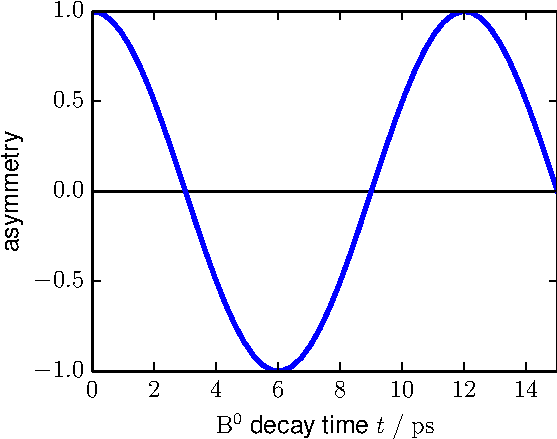
\includegraphics[width=0.8\textwidth]{figures/asym.pdf}
  \end{minipage}
\end{frame}

\begin{frame}{CKM matrix}
  \centering
  Weak eigenstates $\neq$ mass eigenstates\\
  \begin{eqn}
    \begin{pmatrix}
      \Pqd' \\
      \Pqs' \\
      \Pqb' \\
    \end{pmatrix}
    =
    \begin{pmatrix}
      V_{\Pqu\Pqd} & V_{\Pqu\Pqs} & V_{\Pqu\Pqb} \\
      V_{\Pqc\Pqd} & V_{\Pqc\Pqs} & V_{\Pqc\Pqb} \\
      V_{\Pqt\Pqd} & V_{\Pqt\Pqs} & V_{\Pqt\Pqb} \\
    \end{pmatrix}
    \begin{pmatrix}
      \Pqd \\
      \Pqs \\
      \Pqb \\
    \end{pmatrix}
  \end{eqn}

  \begin{itemize}
  \item Conversion via \textbf{C}abibbo \textbf{K}obayashi \textbf{M}askawa matrix
  \item Complex phase $\Rightarrow$ \textit{CP} violation
  \item Unitarity $\Rightarrow$ $\sum_k V_{ik} V_{jk}^* = δ_{ij}$
    $\Rightarrow$ Triangles in the complex plane
  \item Example: $\Vud^{}\Vub^* + \Vcd^{}\Vcb^* + \Vtd^{}\Vtb^* = 0$
  \end{itemize}
\end{frame}

%\begin{frame}{CKM triangle}
%  \centering
%  \begin{tikzpicture}[scale=6]
%    \coordinate (A) at (0.225,0.345); \coordinate (B) at (1,0);
%    \coordinate (C) at (0,0); \node [above] at (0.225,0.365)
%    {$(\bar{ρ},\bar{η})$}; \node [below] at (0, -0.02) {$(0,0)$};
%    \node [below] at (1, -0.02) {$(1,0)$}; \draw (A) -- node[above
%    right] {$\abs{\frac{\Vtd \Vtb^*}{\Vcd \Vcb^*}}$} (B) --
%    node[below] {$1$} (C) -- node[above left] {$\abs{\frac{\Vud
%          \Vub^*}{\Vcd \Vcb^*}}$} (A);
%    \begin{scope}
%      \path[clip] (A) -- (B) -- (C) -- cycle; \draw (A) circle (0.17);
%      \draw (B) circle (0.3); \draw (C) circle (0.19);
%    \end{scope}
%    \node at (0.240,0.260) {$α$}; \node at (0.77,0.045) {$β$}; \node
%    at (0.10,0.06) {$γ$};
%  \end{tikzpicture}
%
%  Idea: overconstrain the apex by performing experiments. \\
%  Inconsistencies would mean New Physics!
%\end{frame}

\begin{frame}{Global CKMfitter results (August 2013)}
  \centering
  \hspace{-2em}
  \begin{tikzpicture}
    \node[anchor=south west,inner sep=0] at (0,0) {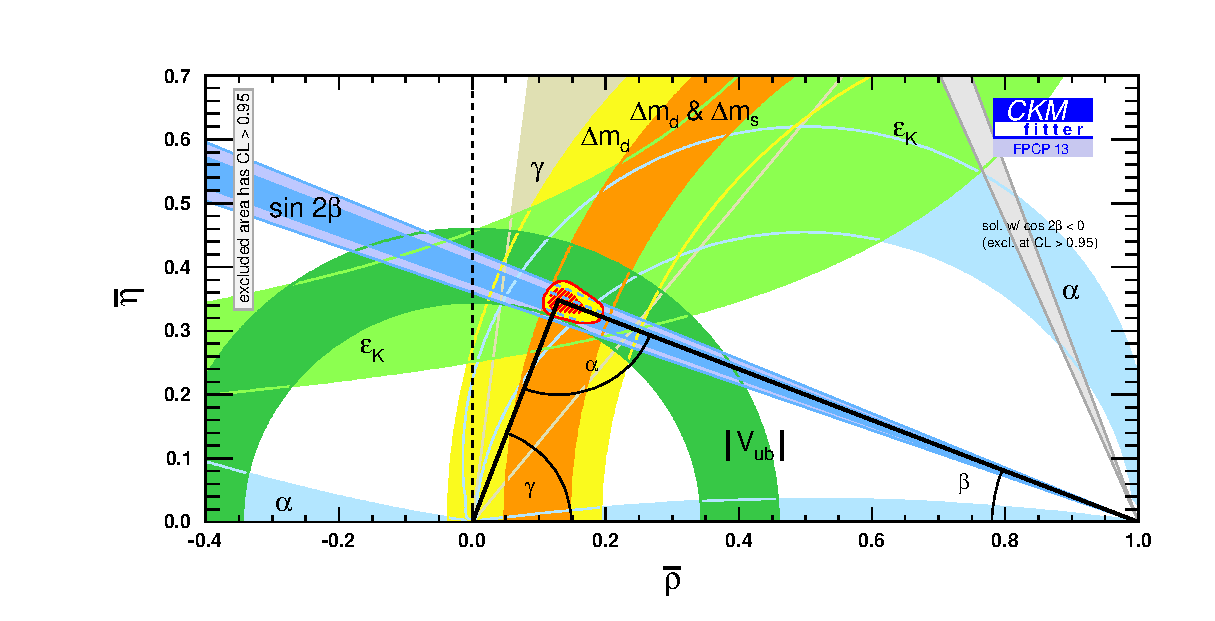
\includegraphics[width=\textwidth]{figures/rhoeta_small_global.eps}};
    \uncover<2>{
      \draw[red,ultra thick,rounded corners] (5,4) rectangle (6.2,4.8);
    }
    \uncover<3>{
      \draw[red,ultra thick,rounded corners] (2.2,3.35) rectangle (3.1,3.9);
    }
  \end{tikzpicture}
  \begin{itemize}
    \item \cite{ckmfitter}
  \end{itemize}
\end{frame}

%\begin{frame}{Motivation: $\difference{m_{\Pqd}}$}
%  Idea: investigate \PBz oscillation to constrain the CKM triangle
%  \begin{itemize}
%  \item Determine $\difference{m_{\Pqd}}$ \\
%    Final state of the \PBz must be known \\
%    $\rightarrow$ Choose channel with self-tagging final state
%  \end{itemize}
%\end{frame}
%
%\begin{frame}{Motivation: $\sin(2β)$}
%  Idea: investigate \PBz oscillation to constrain the CKM triangle
%  \begin{itemize}
%  \item Determine $\sin(2β)$ \\
%    Asymmetry of decay products is caused by CP violation \\
%  \end{itemize}
%  $\Rightarrow$ We need the production state of the \PBz
%\end{frame}

\begin{frame}{LHCb detector}
  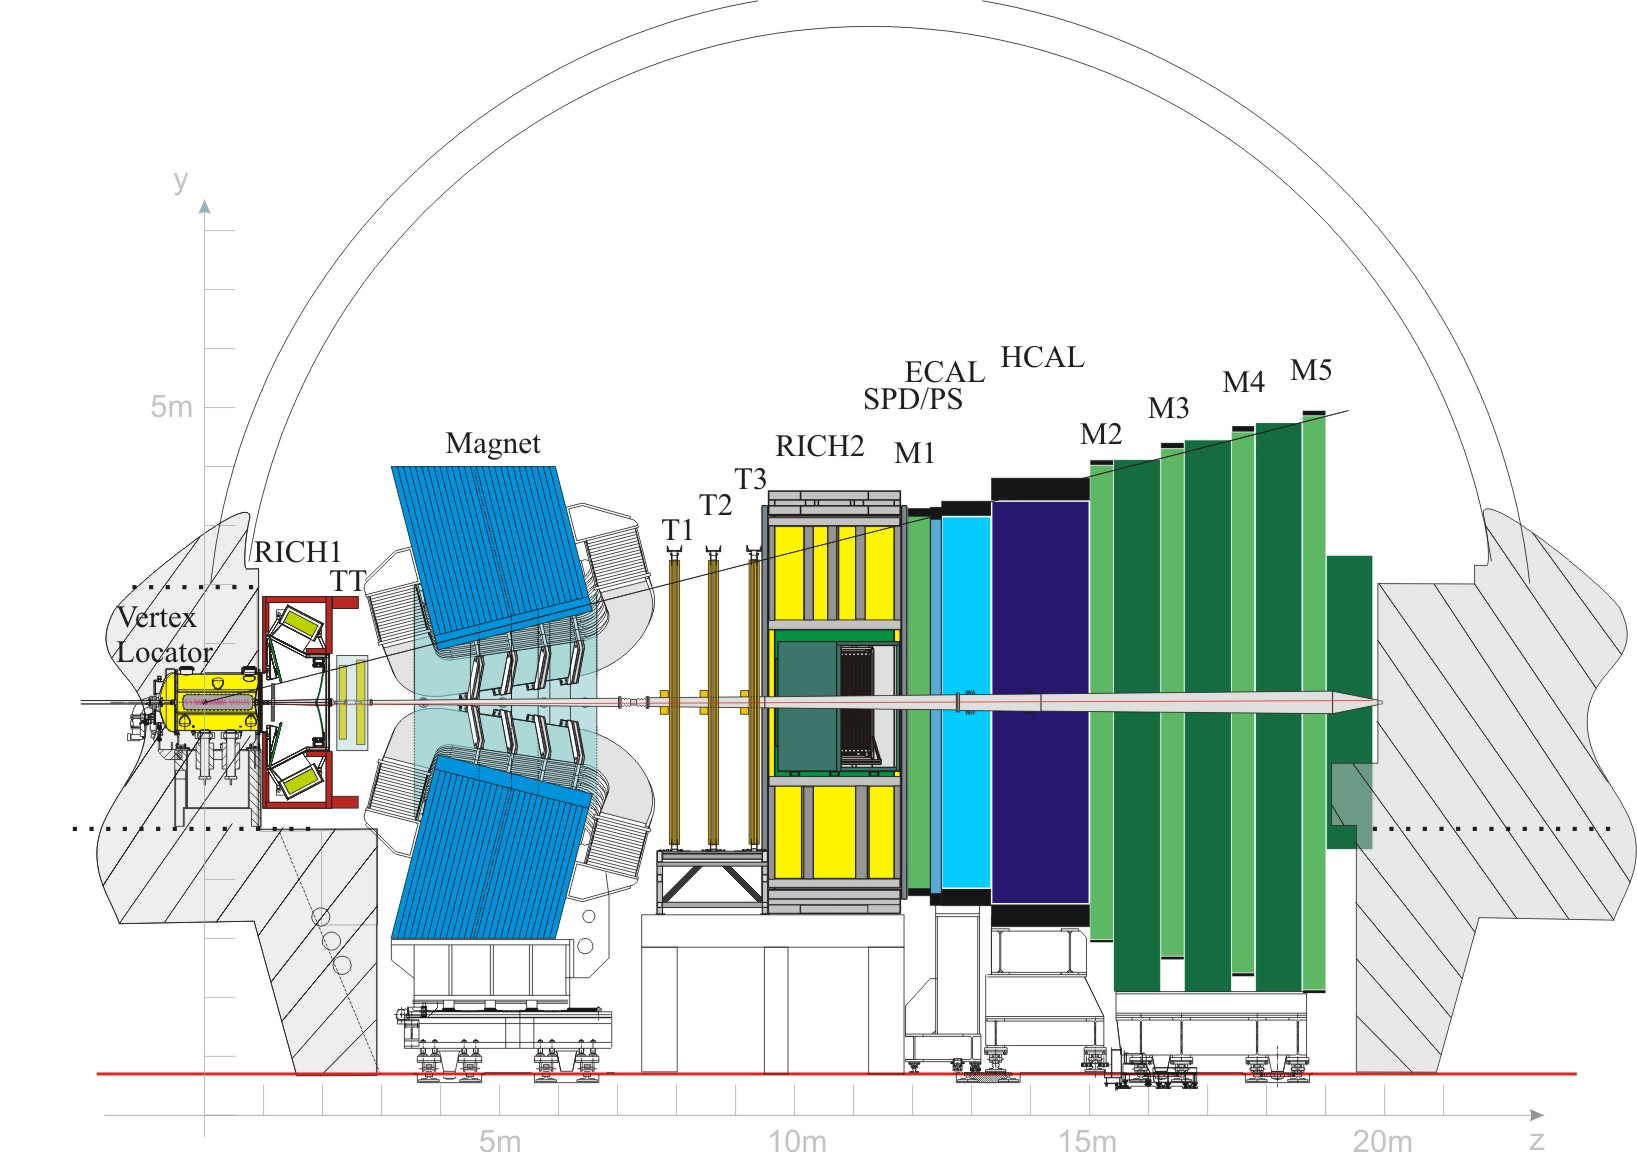
\includegraphics[width=0.9\textwidth]{figures/lhcb.pdf}
  \begin{itemize}
    \item \cite{lhcb}
  \end{itemize}
  % less: what are the components?
  % more: why has it made this analysis possible?
  % pro:
  % designed to detect decays of B mesons
  % great luminosity
  % con:
  % hadronic environment -> difficult to determine initial state of B
  % meson
\end{frame}

\begin{frame}{Flavour tagging}
  \setbeamerfont*{itemize/enumerate body}{size=\footnotesize}
  \begin{itemize}
  \item \small We want to determine the production state of the B meson
  \item \small Can't \enquote{look} at it, must infer by rest of event
  \item \small Idea: Feed event data to neural nets, get tag prediction
  \item \small Two different kinds of strategies: OS, SS
  \end{itemize}
\end{frame}


\begin{frame}{Flavour tagging}
  \centering
  \begin{tikzpicture}[line width=1.2pt,yscale=0.7]
    \begin{overprint}

      % rec
      \draw[dashed,-latex] (1, 0) -- node[above] {\PBz} (5, 2);
      \draw[dashed,-latex] (5, 2) -- (7, 1.5) node[right] {\PKst};
      \draw[dashed,-latex] (5, 2) -- (7, 2.5) node[right] {\PJpsi};

      \uncover<1>{
        \draw[dashed,color=black!40] (1, 0) -- (1, 3);
        \draw[dashed,color=black!40] (5, 2) -- (5, 5);
        \draw[latex-latex] (1, 3) -- node[above] {$\difference{\v{r}}$} (5, 5);
      }

      \uncover<3->{
        \node[right] at (-1, 3) {\textbf{S}ame \textbf{S}ide tagging};
        \draw[solid,-latex] (1, 0) -- (3, 3) node[right] (sshad) {\Pgpp/\PKp};
        \draw[dashed,color=red!40] (sshad) circle (18pt);
      }

      % tag
      \uncover<2->{
        \draw[solid,-latex] (1, 0) -- node[below] {$\PBm$} (3, -1);
        \draw[solid,-latex] (3, -1) -- (5, -3) node[right] (oslepton) {\Pem/\Pmuon};
        \draw[dashed,-latex] (3, -1) -- (5, -2) node[right] {\Pagne/\Pagngm};
        \draw[dashed,-latex] (3, -1) -- (5, -1) node[right] (osd) {\PDz};
        \draw[solid,-latex] (osd.east) -- (7, -1) node[right] (osk) {\PKm};
        \draw[solid,-latex] (osd.east) -- (7, -2) node[right] (ospi) {\Pgpp};
        \draw[dashed,color=red!40] (osk) circle (14pt);
        \draw[dashed,color=red!40] (ospi) circle (12pt);
        \node[right] at (-1, -3) {\textbf{O}pposite \textbf{S}ide tagging};
        \draw[dashed,color=red!40] (oslepton) circle (17pt);
      }

      \uncover<4->{
        \node[above] at (3, 4.5) {This analysis};
        \draw[solid,-latex,color=green] (3, 4.5) -- (3.2, 3.2);
      }

      % interaction
      \node[star,star points=10,fill=orange] (interaction) at (1,0) {};
      \draw[solid,-latex,line width=2pt,color=red] node[left] {\Pp} (0, 0) -- (1, 0);
      \draw[solid,-latex,line width=2pt,color=red] (2.5, 0) node[right] {\Pp} -- (1, 0);

    \end{overprint}
  \end{tikzpicture}
\end{frame}


\begin{frame}{Flavour tagging}
  \begin{itemize}
  \item Problem: tag can't be absolutely accurate $\Rightarrow$ mistag probability $ω$
  \item $ω$ has an effect on the asymmetry! $\rightarrow$ lowers amplitude to $D = (1 - 2 ω)$
  \item $\Rightarrow$ $ω$ has to be extremely well known for $\sin(2β)$
  \item Tagging algorithms (neural nets) can produce mistag estimate $η$
  \end{itemize}
\end{frame}

\begin{frame}{Basic idea of tagging calibration}
  %\item Mistag probability $ω$ must be known precisely
  \begin{enumerate}
    \item Choose a channel with self-tagging final state (\HepProcess{\PBz\to\PJpsi\PKst})
  \item Determine true $ω$ by fitting the data
  \item Find a parameterisation to transform $η$ into $ω$
  \item Reuse that parameterisation when there is no self-tagging final state ($\PBz\to\PJpsi\PKshort$)
  \end{enumerate}
  % But the correct parameterisation depends on the channel.
  % Does this produce accurate results?
\end{frame}

\begin{frame}{Evaluating tagging performance}
  \begin{itemize}
  \item Dilution $D = (1 - 2ω)$
  \item Tagging efficiency $ε_\t{tag} = \frac{N_\t{sig,tagged}}{N_\t{sig}}$
  \item Tagging power $ε_\t{eff} = ε_\t{tag} D^2$
  \end{itemize}
\end{frame}

\begin{frame}{This analysis}
  \centering
  \begin{tikzpicture}[line width=1.2 pt, scale=1]
    \draw[fermion] (0, 2) node[left] {\Pqb} -- (2, 2);
    \draw[fermion] (2, 2) -- (4, 2) node[right] {\Paqc};
    \draw[fermion] (2, 1) -- (4, 1.5) node[right] {\Pqc};
    \draw[fermion] (4, 0.5) node[right] {\Paqs} -- (2, 1);
    \draw[fermion] (0, 0) node[left] {\Pqd} -- (4, 0) node[right] {\Pqd};

    \draw[vector] (1.5, 2) -- node[anchor=north east] {\PW} (2, 1) {};

    \node[left] at (-0.5, 1) {\large\PBz};
    \node[right] at (4.5, 1.8) {\large\PJpsi};
    \node[right] at (4.5, 0.2) {\large\PKst};
  \end{tikzpicture}
  \begin{itemize}
    \item Decay channel: \HepProcess{\PBz\to\PJpsi\PKst}
  \end{itemize}
  \begin{enumerate}
  \item Perform flavour tagging calibration
  \item Apply parameterisation from \HepProcess{\PBz\to\PDm\Pgpp} to \HepProcess{\PBz\to\PJpsi\PKst} \\
        $\rightarrow$ Check by calibrating again. Is $ω\approx η$?
  \end{enumerate}
\end{frame}

\begin{frame}{Dataset}
  \centering
  
\includegraphics[width=0.3\textwidth]{figures/lhcb.jpg}
  \begin{itemize}
  \item Taken at LHCb in 2012: \SI{8}{\tera\electronvolt} CMS energy,
    \SI{2}{\per\femto\barn} luminosity
  \item Relevant variables: mass $m$, decay time $t$, tag decision, final state
    (from Kaon charge)
  \item Also: Mistag prediction $η$
  \item After stripping and offline selection (BDT): ca. \num{5e5}
    event candidates
  \end{itemize}
\end{frame}

\begin{frame}{Analysis - Fitting the data}
  \centering
  \renewcommand{\arraystretch}{0.6}
  \begin{tabular}{c S[table-format=1.2] S[table-format=1.2]}
    \toprule
    category & $η_\t{min}$ & $η_\t{max}$ \\
    \midrule
    1 & 0.40 & 0.50 \\
    2 & 0.35 & 0.40 \\
    3 & 0.30 & 0.35 \\
    4 & 0.25 & 0.30 \\
    5 & 0.00 & 0.25 \\
    \bottomrule
  \end{tabular}
  \vspace{1em}
  \begin{itemize}
  \item Split dataset into five categories depending on $η$
  \item Perform simultaneous maximum likelihood fit over all five categories
  \item Must distinguish between signal and background components
  \item Acceptance and resolution effects taken into account
  \end{itemize}
\end{frame}

\begin{frame}{Analysis - Fit model}
  Probability density function for the fit
  \begin{itemize}
    \item signal:
      \begin{itemize}
        \item mass: triple gaussian
        \item time: exponential with acceptance and oscillation
      \end{itemize}
    \item background (2 components):
      \begin{itemize}
        \item mass: exponential
        \item time: exponential with acceptance
      \end{itemize}
  \end{itemize}
\end{frame}

% TODO mention blinding

\begin{frame}{Analysis - Implementation}
  \begin{itemize}
  \item Decided to re-implement analysis $\rightarrow$ cross-check
  \item Uses Python interface to ROOT and RooFit
  \item $\difference{m_{\Pqd}}$ is blinded
  %\item View of the fit model:
  \end{itemize}
  %\vspace{0.5em}
  %\hspace{-2.5em}
  %
\includegraphics[width=0.98\paperwidth]{figures/model.pdf}
\end{frame}

\begin{frame}[plain]{Results (\enquote{uncalibrated}) - Category 1}
  \centering
  %\hspace{-1.2cm}
  \includegraphics[width=0.39\paperwidth]{analysis/JpsiKst-SSp/plots/Mass-Cat1.pdf}
  \includegraphics[width=0.39\paperwidth]{analysis/JpsiKst-SSp/plots/Time-Cat1.pdf} \\
  %\hspace{-1.2cm}
  \includegraphics[width=0.39\paperwidth]{analysis/JpsiKst-SSp/plots/Mixing-Cat1.pdf}
\end{frame}

\begin{frame}[plain]{Results (\enquote{uncalibrated}) - Category 3}
  \centering
  %\hspace{-1.2cm}
  \includegraphics[width=0.39\paperwidth]{analysis/JpsiKst-SSp/plots/Mass-Cat3.pdf}
  \includegraphics[width=0.39\paperwidth]{analysis/JpsiKst-SSp/plots/Time-Cat3.pdf} \\
  %\hspace{-1.2cm}
  \includegraphics[width=0.39\paperwidth]{analysis/JpsiKst-SSp/plots/Mixing-Cat3.pdf}
\end{frame}

\begin{frame}[plain]{Results (\enquote{uncalibrated}) - Category 5}
  \centering
  %\hspace{-1.2cm}
  \includegraphics[width=0.39\paperwidth]{analysis/JpsiKst-SSp/plots/Mass-Cat5.pdf}
  \includegraphics[width=0.39\paperwidth]{analysis/JpsiKst-SSp/plots/Time-Cat5.pdf} \\
  %\hspace{-1.2cm}
  \includegraphics[width=0.39\paperwidth]{analysis/JpsiKst-SSp/plots/Mixing-Cat5.pdf}
\end{frame}

\begin{frame}{Results (\enquote{uncalibrated})}
  \centering
  \includegraphics[width=0.70\textwidth]{analysis/JpsiKst-SSp/plot.pdf}

  \begin{minipage}{0.45\textwidth}
    \begin{itemize}
    \item $\avg{η} = \num{0.3845 \pm 0.0002}$
    \item $ε_\t{eff} = \SI{0.57 \pm 0.04}{\percent}$
    \end{itemize}
  \end{minipage}
  \begin{minipage}{0.45\textwidth}
    \begin{itemize}
      \item $p_0 = \num{0.432\pm0.004}$
      \item $p_1 = \num{0.82\pm0.10}$
      \item $p_2 = \num{-3.4\pm1.2}$
    \end{itemize}
  \end{minipage}
\end{frame}

\begin{frame}[plain]{Results (\enquote{calibrated}) - Category 1}
  \centering
  %\hspace{-1.2cm}
  \includegraphics[width=0.39\paperwidth]{analysis/JpsiKst-SSp-calibrated/plots/Mass-Cat1.pdf}
  \includegraphics[width=0.39\paperwidth]{analysis/JpsiKst-SSp-calibrated/plots/Time-Cat1.pdf} \\
  %\hspace{-1.2cm}
  \includegraphics[width=0.39\paperwidth]{analysis/JpsiKst-SSp-calibrated/plots/Mixing-Cat1.pdf}
\end{frame}

\begin{frame}[plain]{Results (\enquote{calibrated}) - Category 3}
  \centering
  %\hspace{-1.2cm}
  \includegraphics[width=0.39\paperwidth]{analysis/JpsiKst-SSp-calibrated/plots/Mass-Cat3.pdf}
  \includegraphics[width=0.39\paperwidth]{analysis/JpsiKst-SSp-calibrated/plots/Time-Cat3.pdf} \\
  %\hspace{-1.2cm}
  \includegraphics[width=0.39\paperwidth]{analysis/JpsiKst-SSp-calibrated/plots/Mixing-Cat3.pdf}
\end{frame}

\begin{frame}[plain]{Results (\enquote{calibrated}) - Category 5}
  \centering
  %\hspace{-1.2cm}
  \includegraphics[width=0.39\paperwidth]{analysis/JpsiKst-SSp-calibrated/plots/Mass-Cat5.pdf}
  \includegraphics[width=0.39\paperwidth]{analysis/JpsiKst-SSp-calibrated/plots/Time-Cat5.pdf} \\
  %\hspace{-1.2cm}
  \includegraphics[width=0.39\paperwidth]{analysis/JpsiKst-SSp-calibrated/plots/Mixing-Cat5.pdf}
\end{frame}

\begin{frame}{Results (\enquote{calibrated})}
  \centering
  \includegraphics[width=0.70\textwidth]{analysis/JpsiKst-SSp-calibrated/plot.pdf}
  
  \begin{minipage}{0.45\textwidth}
    \begin{itemize}
    \item $\avg{η_C} = \num{0.4127 \pm 0.0002}$
    \item $ε_\t{eff} = \SI{0.59 \pm 0.04}{\percent}$
    \end{itemize}
  \end{minipage}
  \begin{minipage}{0.45\textwidth}
    \begin{itemize}
      \item $p_0 = \num{0.431\pm0.003}$
      \item $p_1 = \num{0.80\pm0.06}$
    \end{itemize}
  \end{minipage}
\end{frame}

\begin{frame}{Conclusions}
  \begin{itemize}
  \item Calibration successful, parameterisation could be used to improve measurement of $\sin(2β)$
  \item Transference of SS\Pgp calibration parameterisation introduces an error, must be accounted for
  \end{itemize}
\end{frame}

\begin{frame}
  \centering
  \Huge
  Thanks for listening!
\end{frame}

\begin{frame}[shrink=30]{Bibliography}
  \makebibliography
\end{frame}

\appendix
\newcounter{finalframe}
\setcounter{finalframe}{\value{framenumber}}

\begin{frame}[plain]{Results (\enquote{uncalibrated}) - Category 1}
  \centering
  %\hspace{-1.2cm}
  \includegraphics[width=0.39\paperwidth]{analysis/JpsiKst-SSp/plots/Mass-Cat1.pdf}
  \includegraphics[width=0.39\paperwidth]{analysis/JpsiKst-SSp/plots/Time-Cat1.pdf} \\
  %\hspace{-1.2cm}
  \includegraphics[width=0.39\paperwidth]{analysis/JpsiKst-SSp/plots/Mixing-Cat1.pdf}
\end{frame}

\begin{frame}[plain]{Results (\enquote{uncalibrated}) - Category 2}
  \centering
  %\hspace{-1.2cm}
  \includegraphics[width=0.39\paperwidth]{analysis/JpsiKst-SSp/plots/Mass-Cat2.pdf}
  \includegraphics[width=0.39\paperwidth]{analysis/JpsiKst-SSp/plots/Time-Cat2.pdf} \\
  %\hspace{-1.2cm}
  \includegraphics[width=0.39\paperwidth]{analysis/JpsiKst-SSp/plots/Mixing-Cat2.pdf}
\end{frame}

\begin{frame}[plain]{Results (\enquote{uncalibrated}) - Category 3}
  \centering
  %\hspace{-1.2cm}
  \includegraphics[width=0.39\paperwidth]{analysis/JpsiKst-SSp/plots/Mass-Cat3.pdf}
  \includegraphics[width=0.39\paperwidth]{analysis/JpsiKst-SSp/plots/Time-Cat3.pdf} \\
  %\hspace{-1.2cm}
  \includegraphics[width=0.39\paperwidth]{analysis/JpsiKst-SSp/plots/Mixing-Cat3.pdf}
\end{frame}

\begin{frame}[plain]{Results (\enquote{uncalibrated}) - Category 4}
  \centering
  %\hspace{-1.2cm}
  \includegraphics[width=0.39\paperwidth]{analysis/JpsiKst-SSp/plots/Mass-Cat4.pdf}
  \includegraphics[width=0.39\paperwidth]{analysis/JpsiKst-SSp/plots/Time-Cat4.pdf} \\
  %\hspace{-1.2cm}
  \includegraphics[width=0.39\paperwidth]{analysis/JpsiKst-SSp/plots/Mixing-Cat4.pdf}
\end{frame}

\begin{frame}[plain]{Results (\enquote{uncalibrated}) - Category 5}
  \centering
  %\hspace{-1.2cm}
  \includegraphics[width=0.39\paperwidth]{analysis/JpsiKst-SSp/plots/Mass-Cat5.pdf}
  \includegraphics[width=0.39\paperwidth]{analysis/JpsiKst-SSp/plots/Time-Cat5.pdf} \\
  %\hspace{-1.2cm}
  \includegraphics[width=0.39\paperwidth]{analysis/JpsiKst-SSp/plots/Mixing-Cat5.pdf}
\end{frame}

\begin{frame}[plain]{Results (\enquote{calibrated}) - Category 1}
  \centering
  %\hspace{-1.2cm}
  \includegraphics[width=0.39\paperwidth]{analysis/JpsiKst-SSp-calibrated/plots/Mass-Cat1.pdf}
  \includegraphics[width=0.39\paperwidth]{analysis/JpsiKst-SSp-calibrated/plots/Time-Cat1.pdf} \\
  %\hspace{-1.2cm}
  \includegraphics[width=0.39\paperwidth]{analysis/JpsiKst-SSp-calibrated/plots/Mixing-Cat1.pdf}
\end{frame}

\begin{frame}[plain]{Results (\enquote{calibrated}) - Category 2}
  \centering
  %\hspace{-1.2cm}
  \includegraphics[width=0.39\paperwidth]{analysis/JpsiKst-SSp-calibrated/plots/Mass-Cat2.pdf}
  \includegraphics[width=0.39\paperwidth]{analysis/JpsiKst-SSp-calibrated/plots/Time-Cat2.pdf} \\
  %\hspace{-1.2cm}
  \includegraphics[width=0.39\paperwidth]{analysis/JpsiKst-SSp-calibrated/plots/Mixing-Cat2.pdf}
\end{frame}

\begin{frame}[plain]{Results (\enquote{calibrated}) - Category 3}
  \centering
  %\hspace{-1.2cm}
  \includegraphics[width=0.39\paperwidth]{analysis/JpsiKst-SSp-calibrated/plots/Mass-Cat3.pdf}
  \includegraphics[width=0.39\paperwidth]{analysis/JpsiKst-SSp-calibrated/plots/Time-Cat3.pdf} \\
  %\hspace{-1.2cm}
  \includegraphics[width=0.39\paperwidth]{analysis/JpsiKst-SSp-calibrated/plots/Mixing-Cat3.pdf}
\end{frame}

\begin{frame}[plain]{Results (\enquote{calibrated}) - Category 4}
  \centering
  %\hspace{-1.2cm}
  \includegraphics[width=0.39\paperwidth]{analysis/JpsiKst-SSp-calibrated/plots/Mass-Cat4.pdf}
  \includegraphics[width=0.39\paperwidth]{analysis/JpsiKst-SSp-calibrated/plots/Time-Cat4.pdf} \\
  %\hspace{-1.2cm}
  \includegraphics[width=0.39\paperwidth]{analysis/JpsiKst-SSp-calibrated/plots/Mixing-Cat4.pdf}
\end{frame}

\begin{frame}[plain]{Results (\enquote{calibrated}) - Category 5}
  \centering
  %\hspace{-1.2cm}
  \includegraphics[width=0.39\paperwidth]{analysis/JpsiKst-SSp-calibrated/plots/Mass-Cat5.pdf}
  \includegraphics[width=0.39\paperwidth]{analysis/JpsiKst-SSp-calibrated/plots/Time-Cat5.pdf} \\
  %\hspace{-1.2cm}
  \includegraphics[width=0.39\paperwidth]{analysis/JpsiKst-SSp-calibrated/plots/Mixing-Cat5.pdf}
\end{frame}

\begin{frame}[plain]{Correlation matrices}
  \begin{minipage}{0.48\textwidth}
  \includegraphics[width=\textwidth]{analysis/JpsiKst-SSp/quadratic-correlation.pdf}
  \begin{itemize}
    \item \enquote{uncalibrated} - quadratic
  \end{itemize}
  \end{minipage}
  \begin{minipage}{0.48\textwidth}
  \includegraphics[width=\textwidth]{analysis/JpsiKst-SSp-calibrated/linear-correlation.pdf}
  \begin{itemize}
    \item \enquote{calibrated} - linear
  \end{itemize}
  \end{minipage}
\end{frame}

\setcounter{framenumber}{\value{finalframe}}
\end{document}



\end{document}
